\chapter{Discussion}
\label{chapter:conclusion}

    %% TODO
    %% - SimGrid suppose que les consommations réseau et cpu sont linéaires
    %%   et indépendantes. Ce n'est pas si simple. Tension entre
    %%   mesurer/injecter et modéliser/prédire.
    %% - Ça marche mais niveau d'expertise encore assez démentiel
    %% - Résolution/automatisation de pas mal de choses en terme de
    %%   modélisation de plate-forme mais il y a encore beaucoup de
    %%   travail. LibSimBLAS ?

    \section{Contribution}%

        This thesis has contributed to the improvement of experimental reproducibility in high performance computing.

        In Part~\ref{part:prediction}, we described a method for predicting the performance of MPI applications through
        simulation. Using Simgrid/SMPI simulator, we managed to emulate the High Performance Linpack benchmark at scale
        by applying only a few modifications to its source code. We compared several computation and communication
        models and showed the importance of modeling both the temporal and spatial variability of the platform. In a
        thorough comparison of the simulations with real executions, we show that the prediction error remains very low,
        only a few percent, thereby demonstrating the faithfulness of this approach. Several sensibility analyses are
        then performed to quantify the effect of platform variability and showcase an important use case of simulation.

        The lessons learned during this work are then presented in Part~\ref{part:experiment}. We start by describing the
        experiment engine we developed and that was used throughout this thesis. Then, we present an in-depth report of
        the many experimental biases we faced, including very unsettling phenomenons we did not anticipate. While some
        of these biases can be desirable if they are also occurring in the simulated application, most of them had to be
        suppressed through randomization. Finally, we showcase the performance non-regression test we implemented. While
        not a statistical novelty, they allowed us to detect many changes on Grid'5000 platform that affected
        significantly the performance and could harm experiments if gone unnoticed. We believe the HPC community could
        greatly benefit of such tests.

    \section{Trusting our predictions}%
    \label{sec:prediction_trust}

        Unlike mathematical theorems or algorithms, the correctness of a model like those of Part~\ref{part:prediction}
        cannot be formally proven. The only sound method for validating its faithfulness is to thoroughly try to break
        it, by comparing predictions to reality while methodically changing the configurations. As presented in
        Chapter~\ref{chapter:prediction:validation}, we did cover an extensive range of configurations in our
        validation. Before managing to systematically obtain accurate predictions, we stumbled on many problems which
        caused our predictions to be unrealistic. We had to investigate, understand and overcome these multiple
        obstacles, as reported in Part~\ref{part:experiment}.

        A few weeks before the defense of this thesis, we decided to repeat the whole simulation study from scratch on
        another Grid'5000 cluster named \gros, using 60 of its nodes. This cluster has different nodes (one Intel Xeon
        Gold 5220 processor per node with \NSI{96}{\giga\byte} of memory), a different network (with
        \NSI{25}{\giga\bit/\second} Ethernet) and we used a more recent version of OpenBLAS (resulting in the use of
        AVX512 instructions by the \dgemm function instead of AVX2). Over the course of a weekend, we calibrated the
        platform by measuring the \dgemm and MPI durations. Then, we performed real and simulated HPL executions. At
        first, the predicted performance was too low by one order of magnitude. This was due to a mistake we made: we
        computed the linear regression of the \dgemm model using all the terms of the polynomial, even those of degree
        one (\ie \(M\), \(N\) and \(K\)) which were not statistically significant. This resulted in an overfitted model
        with spurious predictions.  After fixing this issue by only considering the significant terms, we obtained
        extremely accurate predictions of HPL performance for various matrix sizes (see
        Figure~\ref{fig:conclusion:gros_study}).

        \begin{figure}[htpb]
            \centering
            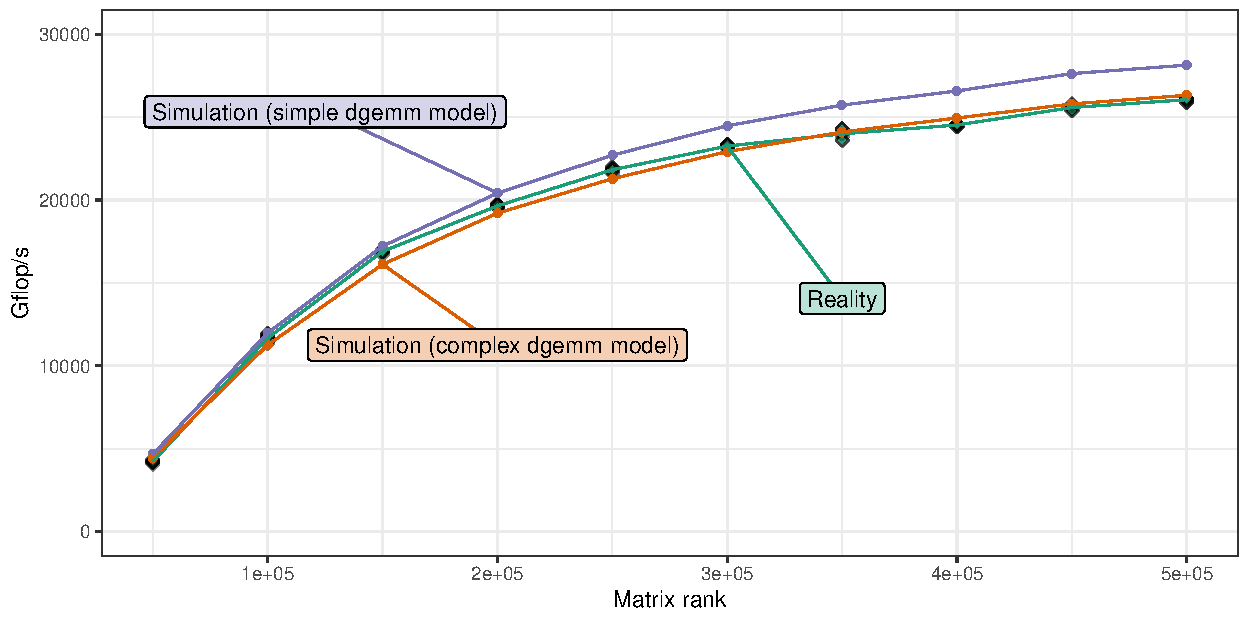
\includegraphics[width=\linewidth]{img/conclusion/validation_gros.pdf}
            \caption{HPL performance: prediction vs. reality for various matrix ranks, using 60 nodes of the \gros
            cluster.}%
            \label{fig:conclusion:gros_study}
        \end{figure}

        Similarly to what we observed in Chapter~\ref{chapter:prediction:validation}, the predictions are more accurate
        with a complex \dgemm model (\ie heterogeneous, stochastic and polynomial)  than with a simpler model (\ie
        homogeneous, deterministic and linear). However, the simpler model still makes reasonably low prediction errors
        here as the \gros cluster has less variability than the \dahu cluster.

        This small additional study demonstrates clearly the level of trust we can now have in our model, but also its
        fragility, as seemingly inoffensive changes in the approach can lead to widely inaccurate predictions.

    \section{Future work}%

        Besides the next steps already discussed in Chapter~\ref{chapter:prediction:conclusion} and
        Section~\ref{sec:test:conclusion}, there also remains a unification work. By going a step further in the
        automation, we could use the data produced by the non-regression tests to generate new model instances for
        Simgrid. It would then be possible to make new simulations with a platform model that reflects the latest
        changes of the real platform. Then, by implementing the same statistical test on the performance predicted by
        the simulation, we should be able to detect whether a platform change has affected the application
        performance and quantify this effect. A minor performance drop of the computation kernels could be amplified by
        the synchronization phases of the application and become very concerning at a larger scale. Conversely, it could
        also be attenuated by the global noise and go completely unnoticed.

        We believe that our predictions could be extremely valuable to the whole life cycle of supercomputers:
        \begin{description}
            \item[Design] Using simulations, manufacturers could apply co-design techniques to construct the most
                performant machines for a given set of target applications and within a given budget. This could help
                achieve more faithful results than the current techniques relying on less accurate simulations or even
                guesswork.
            \item[Development] Simulations could also largely benefit software developers. Both debugging and tuning the
                application are more convenient and less expensive in simulation than in reality, especially if large
                scale runs are required.
            \item[Maintenance] Whenever the platform employees need to perform some maintenance, there is a
                non-negligible risk of affecting the machine performance, as we illustrated in
                Chapter~\ref{chapter:experiment:tests}. To verify that the performance did not change, the usual method
                is to perform large-scale runs of a benchmark such as HPL, which can largely lengthen the maintenance
                duration. A more convenient alternative would be to (1) carry small but carefully designed performance
                tests as those described in Chapter~\ref{chapter:experiment:tests} to check if there is anything
                obviously wrong, and (2) perform large-scale simulations with the updated model and compare the new
                predictions with the previous ones.
        \end{description}
